% 
% Annual CCN conference
% Sample LaTeX Two-Page Summary -- Proceedings Format
% based on the prior cognitive science style file

% Original : Ashwin Ram (ashwin@cc.gatech.edu)       04/01/1994
% Modified : Johanna Moore (jmoore@cs.pitt.edu)      03/17/1995
% Modified : David Noelle (noelle@ucsd.edu)          03/15/1996
% Modified : Pat Langley (langley@cs.stanford.edu)   01/26/1997
% Latex2e corrections by Ramin Charles Nakisa        01/28/1997 
% Modified : Tina Eliassi-Rad (eliassi@cs.wisc.edu)  01/31/1998
% Modified : Trisha Yannuzzi (trisha@ircs.upenn.edu) 12/28/1999 (in process)
% Modified : Mary Ellen Foster (M.E.Foster@ed.ac.uk) 12/11/2000
% Modified : Ken Forbus                              01/23/2004
% Modified : Eli M. Silk (esilk@pitt.edu)            05/24/2005
% Modified : Niels Taatgen (taatgen@cmu.edu)        10/24/2006
% Modified : David Noelle (dnoelle@ucmerced.edu)     11/19/2014
% Modified : Konrad Kording (koerding@gmail.com)     2/15/2017
% Modified : Thomas Naselaris (tnaselar@gmail.com)   3/18/2022
% Modified : Sneha Aenugu & Jasper van den Bosch   18/12/2024

\documentclass[10pt,letterpaper]{article}

\usepackage{ccn}
\usepackage{pslatex}
\usepackage{apacite}
\usepackage{graphicx}
\usepackage{hyperref}
\hypersetup{colorlinks=false,breaklinks=true}
\usepackage{natbib}


\title{How far have deep learning models come on visual reasoning?}

% \author{{\large \bf Anonymous authors} \\
% Double blind review}

% \author{{\large \bf Brian Kim (brian_kim@alumni.brown.edu)} \\
% Brown University}
 
% \author{{\large \bf Siyu Zeng (siyu_zeng1@brown.edu)} \\
%   Brown University }\\
% A City, State 12345 A country
%   \AND {\large \bf Another Person (AnotherPerson@this.planet.edu)} \\
%   A Department, 1234 Example Street\\
% A City, State 12345 A country}


\begin{document}

\maketitle


% ORIGINAL ABSTRACT:
% Deep neural networks today rival humans on most visual tasks. Here, we investigate whether these gains in accuracy have also endowed models with the capabilities to solve simple visual reasoning tests. We benchmark 1,259 pretrained models on two visual reasoning tasks, Pathfinder and cluttered ABC, using linear probes to test whether representations learned for image classification generalize to these settings. We find that most of the models struggle to generalize to these tasks. However, the most recent and largest-scale visual transformers break trend and show an accelerating relationship between ImageNet accuracy and visual reasoning capabilities. These findings suggest that we may be entering a new phase of deep learning for vision science, in which models with billions (or trillions) of synapses trained on large proportions of internet images automatically discover mechanisms that are necessary for visual reasoning even without explicit training for such capabilities.

\begin{abstract}
% PREVIOUS ABSTRACT:
% Deep neural networks have made rapid progress on visual recognition, but do their learned representations support visual reasoning---the ability to trace contours, group elements, and resolve spatial relationships? Prior work has shown that both CNNs and transformers struggle on tasks like Pathfinder even when trained from scratch on millions of examples \citep{Serre2018a,Serre2018b}, and the Long Range Arena benchmark found that no transformer variant could learn Pathfinder reliably \citep{LRA}. Here, we ask a different question: can models that were never trained on such tasks nonetheless solve them, by virtue of large-scale pretraining on natural images? We benchmark 1,259 pretrained models from the TIMM library on Pathfinder and cluttered ABC (cABC), using linear probes on frozen representations. Most models fail as the required reasoning range increases. However, the largest and most recent Vision Transformers break this trend, showing a strengthening relationship between ImageNet accuracy and visual reasoning performance. These results suggest that large-scale pretraining may give rise to long-range reasoning capabilities that explicit training on such tasks could not---with implications for both architecture design and the use of deep networks as models of biological vision.
Large-scale pretraining has become the dominant paradigm in computer vision, but do the representations it produces support visual reasoning---the ability to trace contours, group elements, and resolve spatial relationships? These capabilities have proven remarkably difficult to learn: neither CNNs nor transformers could solve benchmarks like Pathfinder when trained directly on millions of examples \citep{Serre2018a,Serre2018b,LRA}. Here, we ask whether large-scale pretraining on natural images succeeds where supervised training on these tasks does not. We probe 1,259 pretrained models from the TIMM library on Pathfinder and cluttered ABC (cABC), using linear readouts from frozen representations. Most models fail as the required reasoning range increases. However, the largest and most recent Vision Transformers break this trend, showing a strengthening relationship between ImageNet accuracy and visual reasoning performance. These results suggest that large-scale pretraining may give rise to long-range reasoning capabilities that explicit training could not---with implications for architecture design and the use of deep networks as models of biological vision.
\end{abstract}

% ORIGINAL INTRO:
% Long-range reasoning is a fundamental component of visual tasks ranging from tracing to grouping and segmentation. Theories of visual perception have proposed a distinction between parallel, feedforward grouping of local features and serial, attention-demanding grouping of spatially distant elements \citep{Houtkamp}. Current vision models are typically optimized for tasks that may depend more on feedforward processing: for example, object recognition, scene classification, and other benchmarks where local features carry most of the discriminative signal. Whether these models also learn long-range reasoning capabilities remains an open question.
%
% Benchmarks designed to isolate long-range reasoning in humans and machines include Pathfinder \citep{Serre2018a, Serre2018b}, which was also incorporated into the Long-Range Arena \citep{LRA}, and the cluttered ABC (cABC) task. Both parametrically control the spatial range over which reasoning must occur, making them well-suited for measuring how and when models fail. However, the landscape of vision architectures has expanded considerably since those benchmarks were introduced. Vision Transformers \citep{Dosovitskiy} introduced global self-attention over image patches, and state-space models \citep{Gu} extended recurrent architectures to long sequences---both offering, in principle, the capacity to model long-range spatial dependencies that CNNs lack by construction.
%
% However, it is unclear whether these architectural advances have translated into genuine long-range reasoning ability, or whether they simply provide better local features and more capacity. In this paper, we test this question by evaluating 1,259 pretrained models from the TIMM library \citep{Wightman}, on Pathfinder and cABC at multiple difficulty levels. Using linear probes on frozen representations from these models, we test whether features learned for image classification generalize to long-range reasoning without further training. We find that most models struggle more as the spatial extent of reasoning increases. However, the largest and most recent Vision Transformers break this trend, exhibiting a strengthening relationship between ImageNet accuracy and visual reasoning performance. These results suggest that large-scale pretraining routines used in state-of-the-art models have unlocked new capabilities for long-range reasoning, and a continuation of this scale-up may lead to human-level visual reasoning performance even without explicit training on such tasks---a result with implications for both architecture design and the use of DNNs as models of biological vision.

\section{Introduction}
Visual reasoning---tracing contours, grouping elements, resolving spatial relationships---requires integrating information across distant locations in the visual field. Theories of visual perception draw a distinction between parallel, feedforward grouping of local features and serial, attention-demanding grouping of spatially distant elements \citep{Houtkamp}. Most vision models are optimized for tasks like object recognition and scene classification, where local features carry the discriminative signal. Whether these models also acquire long-range reasoning capabilities, particularly through large-scale pretraining, is an open question.

Prior work suggests they should not. Benchmarks designed to isolate long-range reasoning---Pathfinder \citep{Serre2018a, Serre2018b} and cluttered ABC (cABC)---parametrically control the spatial range over which reasoning must occur. Neither CNNs nor transformers could solve these tasks when trained directly, even with millions of examples; the Long-Range Arena confirmed that no transformer variant learned Pathfinder reliably \citep{LRA}. Since then, the architectural landscape has expanded: Vision Transformers \citep{Dosovitskiy} introduced global self-attention over image patches, and state-space models \citep{Gu} extended recurrent architectures to long sequences. Both offer, in principle, the capacity for long-range spatial interaction that CNNs lack. But it remains unclear whether these advances translate into genuine reasoning ability, or simply provide better features and more capacity.

We test this by probing 1,259 pretrained models from the TIMM library \citep{Wightman} on Pathfinder and cABC at multiple difficulty levels, using linear readouts from frozen representations.

% \begin{figure}[ht]
% % \begin{center}
% % \fbox{CCN figure}
% % \end{center}
% 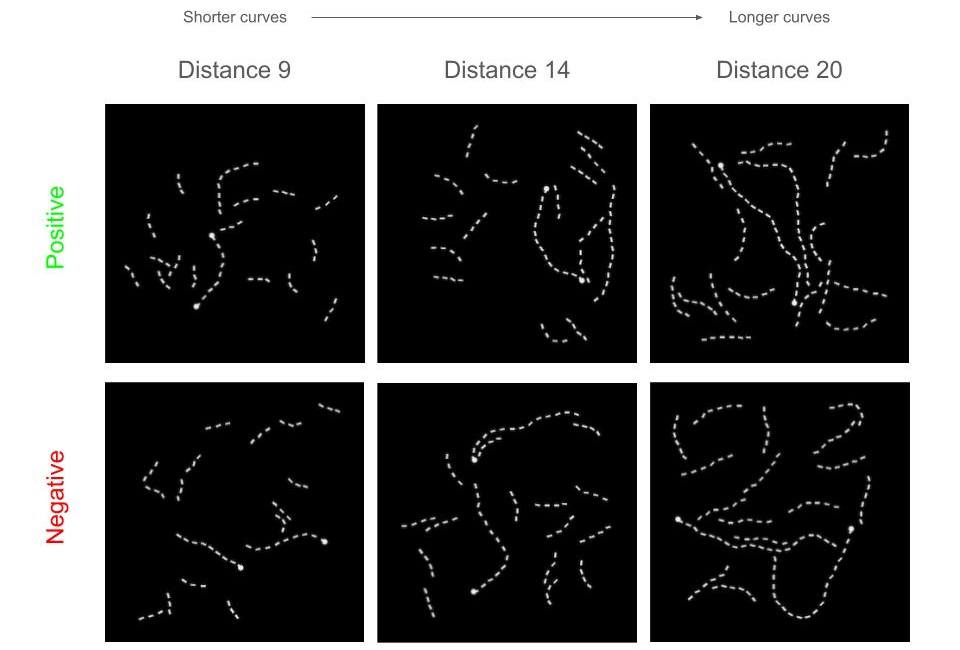
\includegraphics[width=\linewidth]{PF ex.jpg}
% \caption{In the Pathfinder task, participants must determine whether two white markers fall on the same or different path. The difficulty of this task is parametrically controlled by the length of the target curve.} 
% \label{Pathfinder-Graphic}
% \end{figure}

% \begin{figure}[ht]
% % \begin{center}
% % \fbox{CCN figure}
% % \end{center}
% 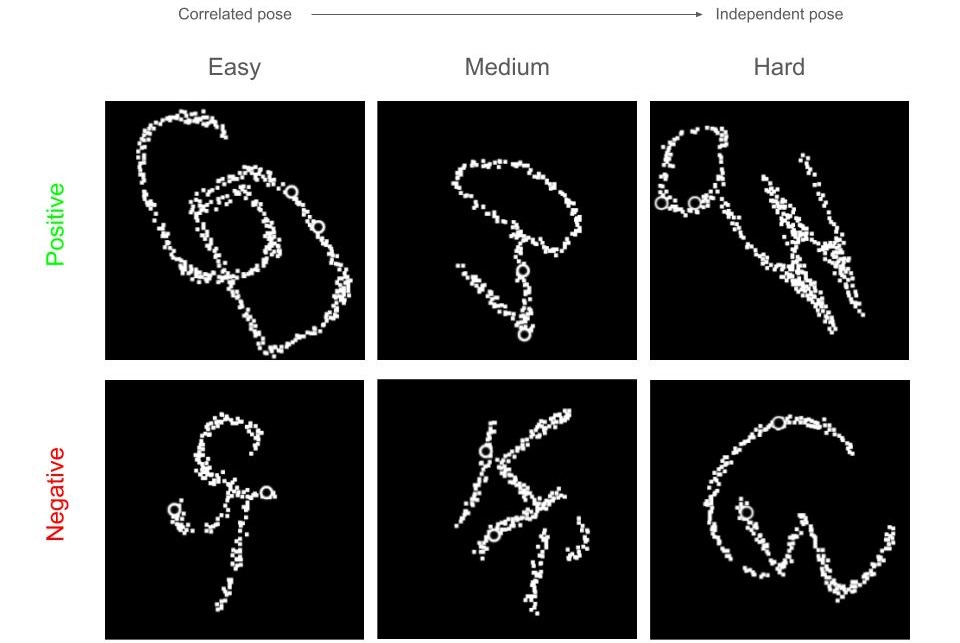
\includegraphics[width=\linewidth]{cABC ex.jpg}
% \caption{In the cABC task, participants must determine whether two white markers fall on the same or different letter. The difficulty of this task is parametrically controlled by decreasing the correlation between geometric transformations applied to the two letters while increasing the
% relative positional variability between letters.} 
% \label{cABC-Graphic}
% \end{figure}

\section{Methods}

\textbf{Models.} We sourced 1,259 pretrained models from the PyTorch Image Models (TIMM) library \citep{Wightman}, spanning four architecture families: convolutional neural networks (CNNs), Vision Transformers (ViTs), convolutional-transformer hybrids (ConvViTs), and recurrent neural networks (RNNs). All models were pretrained for image classification and their weights were frozen during evaluation.

\textbf{Tasks.} We evaluated models on two visual reasoning challenges designed to parametrically control the spatial range over which reasoning must occur. In Pathfinder, participants judge whether two white markers lie on the same or different curve; difficulty increases with curve length. In the cluttered ABC (cABC) task, participants judge whether two markers fall on the same or different letter; difficulty increases with the independence in alignment and orientation between letters. For both tasks, we trained and evaluated linear probes at each difficulty level independently, allowing us to track how performance is affected by the required spatial range of reasoning.
% and addressing recent concerns on fixed-difficulty long-range benchmarks \citep{Miralles}.

\textbf{Evaluation.} For each model, we extracted frozen penultimate-layer representations and trained a linear probe to classify stimuli at each difficulty level. Linear probing was chosen for two reasons. First, it allowed us to scale evaluation across the full set of 1,259 models. Second, training from scratch has been shown to overestimate architectural differences \citep{Amos}; probing pretrained representations instead directly tests whether features learned for image classification generalize to long-range visual reasoning.

% \begin{figure*}[ht]
\begin{figure*}[!ht]
% \begin{center}
% \fbox{CCN figure}
% \end{center}
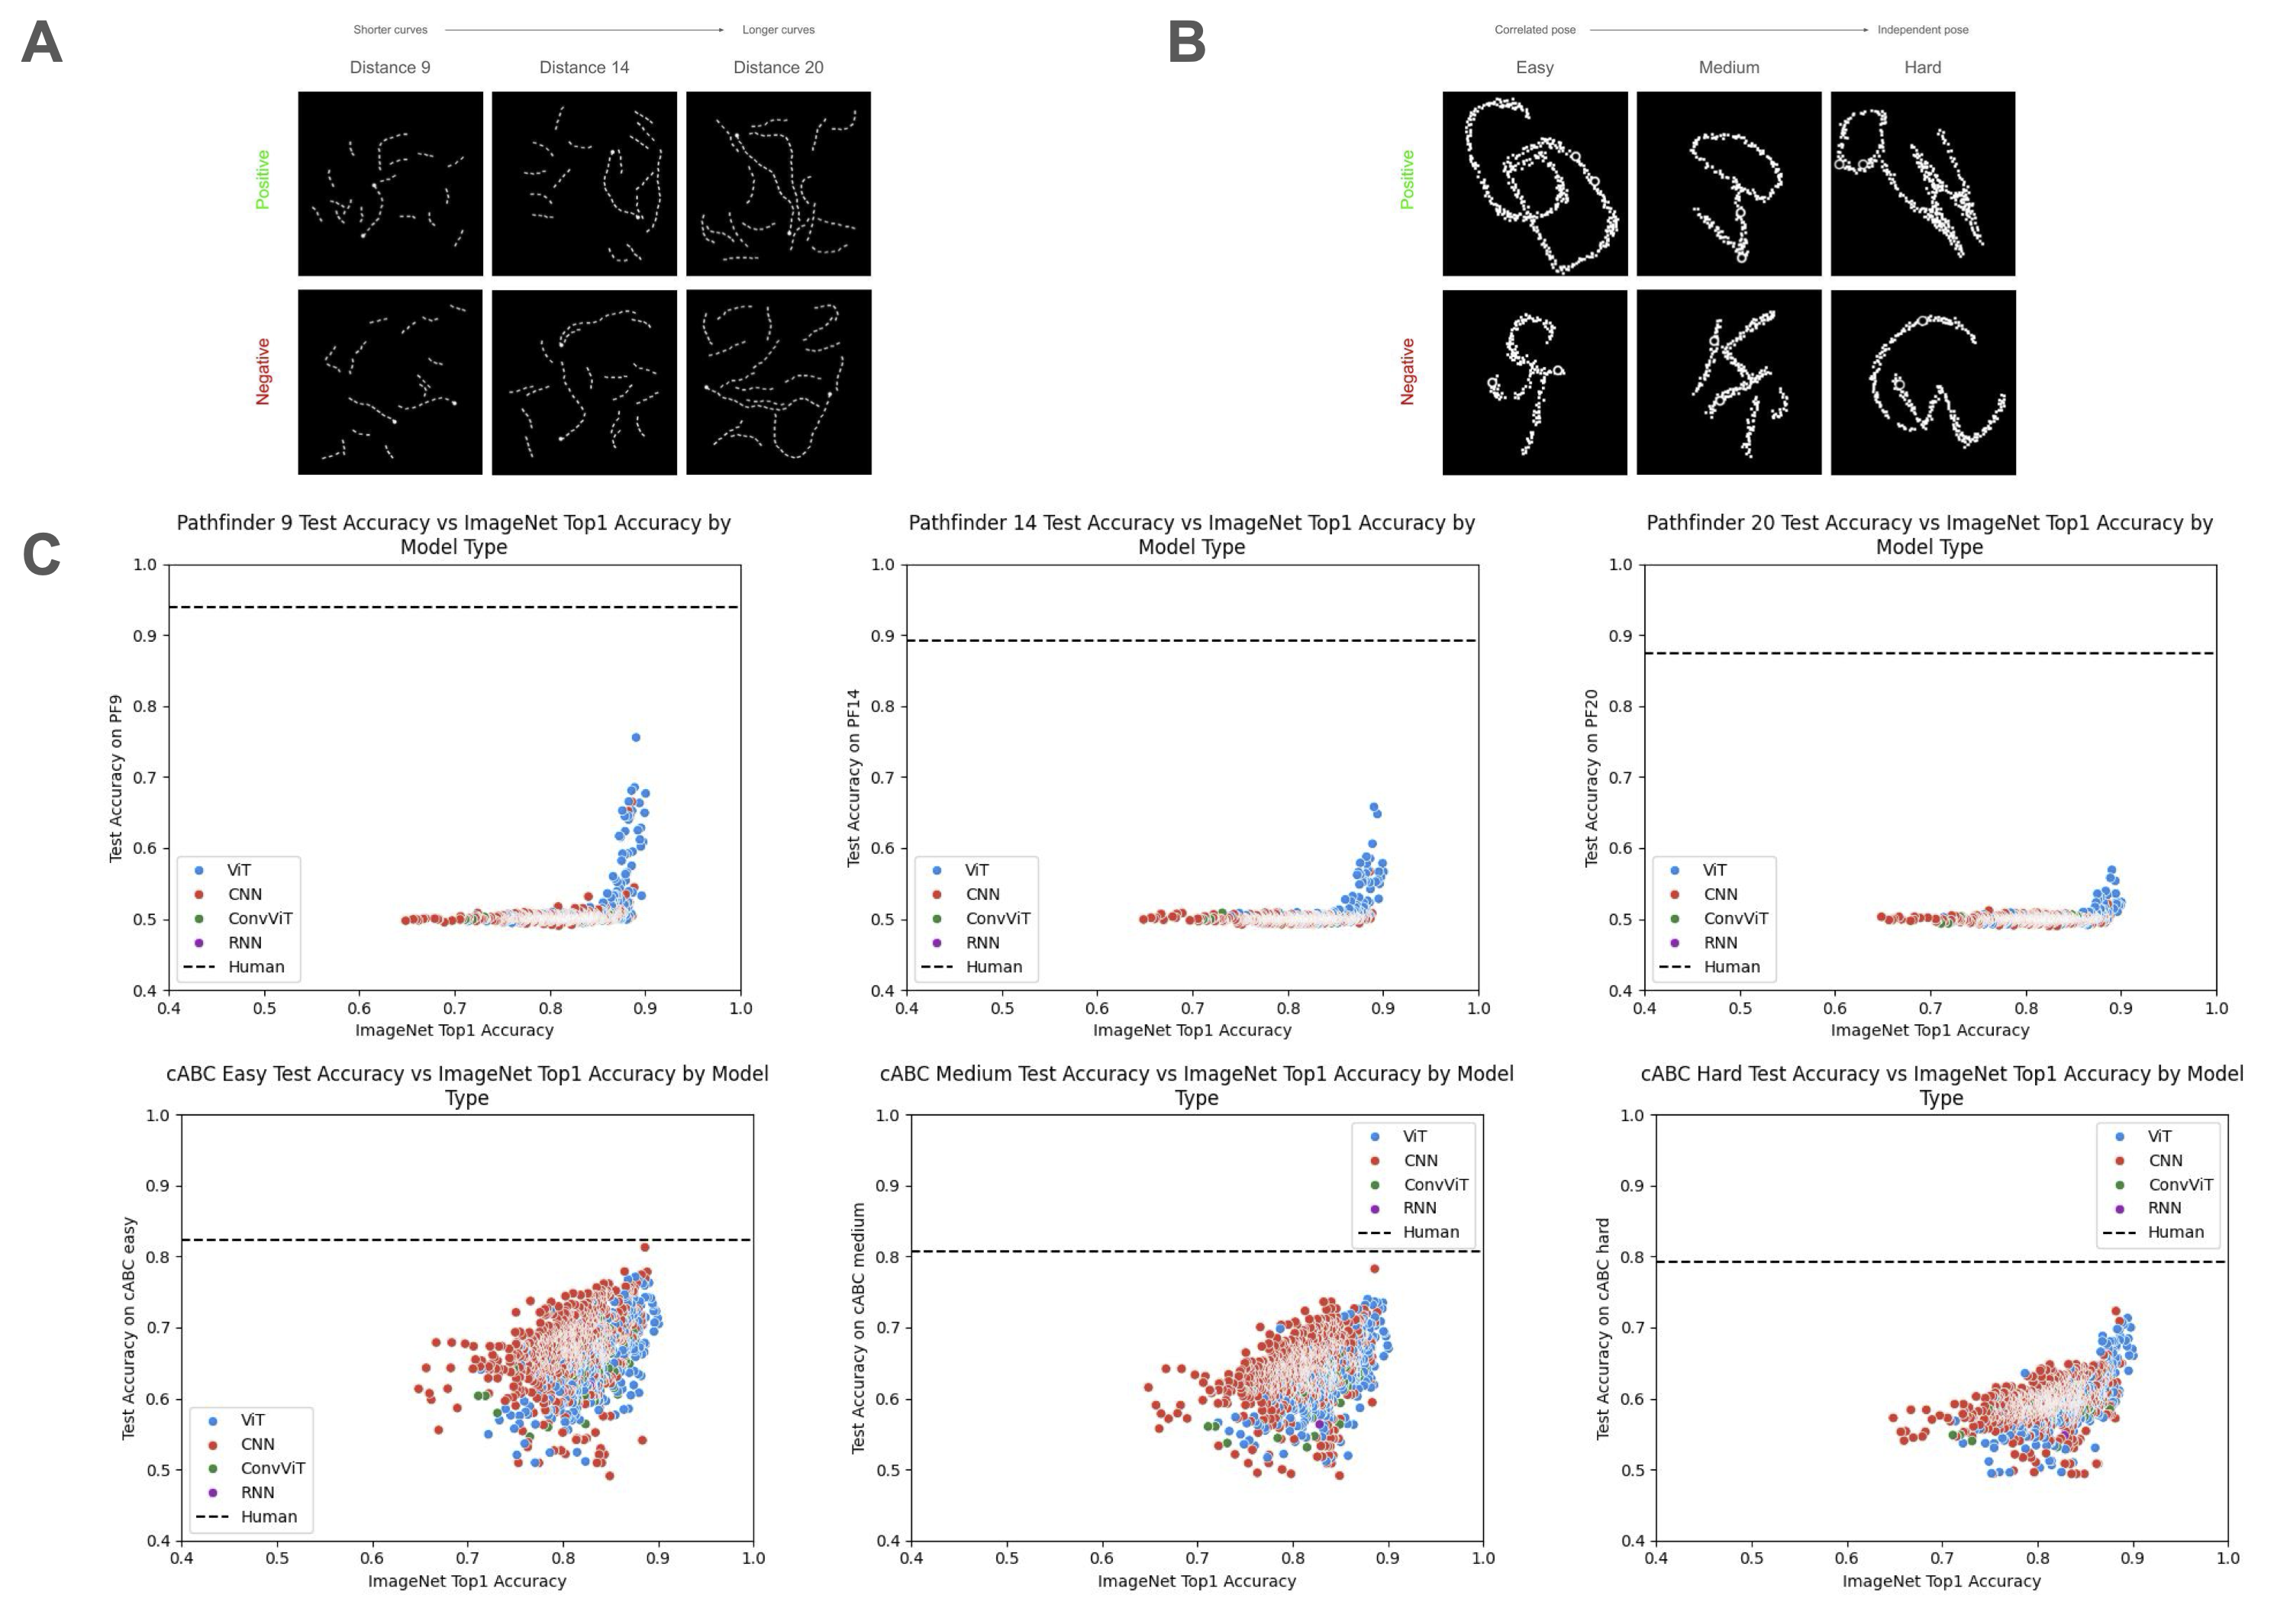
\includegraphics[width=\textwidth]{PF_cABC_Reorder.png}
\caption{\textbf{Model performance on PathFinder and cABC challenges. }\textbf{A.} Examples of PathFinder, where participants must determine whether two white markers fall on the same or different path. \textbf{B.} Examples of cABC, where participants must determine whether two white markers fall on the same or different letter. \textbf{C.} On both challenges, model performance (p = 1259) noticeably decreased as the difficulty of the task---a control for the distance in the long-range reasoning required for the task\textemdash increased, indicating that models struggle to generalize to longer-range reasoning problems after being trained on natural images.}
% decreasing the correlation between geometric transformations applied to the two letters while increasing the relative positional variability between letters.} 
% \caption{When breaking down model performances across the Pathfinder and cABC tasks, model performance in aggregate (p = 1259) noticeably decreased as the difficulty of the task – an indication of the distance in the long-range reasoning required for the task – increased. This pattern is most apparent in the Pathfinder task, which also saw better-than-random performance exclusively at those models which had the highest ImageNet accuracy, here using Top1 performance as a loose proxy for model size. cABC showed broader above-chance performance that nevertheless degraded with difficulty.} 
\label{Zoo-Results}
\end{figure*}

\section{Results}

Across both tasks, aggregate model performance declined as difficulty increased, confirming that the spatial range of reasoning is a key bottleneck for pretrained vision models (Fig.~\ref{Zoo-Results}a). However, the severity and pattern of this decline differed markedly between tasks.

On Pathfinder, models achieved above-chance accuracy at the lowest difficulty, but performance collapsed to near-random levels at the highest difficulty across nearly all 1,259 models. Critically, the few models that achieved above-chance performance at higher difficulties were exclusively those with the highest ImageNet Top-1 accuracy—predominantly large-scale ViTs. CNNs were uniformly weak across all Pathfinder difficulty levels. Transformer-based architectures fared better, though performance still degraded as the required range grew.

On cABC, models performed significantly better overall, and the decline with difficulty was more gradual. A broader range of architectures, including CNNs, achieved above-chance performance even at higher difficulty levels. Nevertheless, CNNs exhibited the steepest drop-off as difficulty increased, mirroring the architectural pattern observed in Pathfinder.

% ORIGINAL CONCLUSION:
% Together, these results demonstrate that most pretrained vision models fail to encode long-range spatial relationships, even when they achieve high accuracy on standard classification benchmarks. The exceptions are the largest and most recent Vision Transformers, which suggest a superlinear relationship between ImageNet accuracy and visual reasoning performance—suggesting that sufficient scale and modern pretraining may give rise to long-range reasoning capabilities without explicit training on such tasks.

\section{Conclusion}

Most pretrained vision models fail to encode long-range spatial relationships, even when they achieve high accuracy on standard classification benchmarks. The exceptions are the largest and most recent Vision Transformers, which show a strengthening relationship between ImageNet accuracy and visual reasoning performance. This suggests that sufficient scale and modern pretraining may give rise to long-range reasoning capabilities without explicit training.

From a neuroscience perspective, these findings speak to a longstanding distinction between feedforward and recurrent processing in biological vision \citep{Houtkamp}. Tasks like Pathfinder are thought to require iterative, potentially recurrent computation in the visual cortex. The fact that only the largest transformers---with global self-attention over the full image---succeed where CNNs uniformly fail is consistent with this view: architectural capacity for long-range interaction appears necessary, and local feature extraction is not sufficient. Whether these models solve such tasks through mechanisms that parallel biological recurrence or through qualitatively different strategies remains an open question for future work.

% Figure~\ref{sample-figure}. If necessary, leave extra white space at
% the bottom of the page to avoid splitting the figure and figure
% caption. You may float figures to the top or bottom of a column, or
% set wide figures across both columns.


% \section{Acknowledgments (camera-ready version only)}
% Please refrain from adding acknowledgments to the double-blind version to protect anonymity. Include acknowledgments \textbf{only} in the final accepted version of the manuscript. 



\bibliographystyle{ccn_style}

\setlength{\bibleftmargin}{.125in}
\setlength{\bibindent}{-\bibleftmargin}

\bibliography{ccn_style}


\end{document}
